\documentclass{easychair}

\usepackage{doc}

\title{Where is the web still insecure? \\ Regional scans for HTTPS 
certificates}

\author{
    Anushah Hossain \inst{1}
\and
    Kristina Nelson \inst{1}
\and
    Tjerand Silde \inst{1,} \inst{2} \thanks{The author presented this paper at the NISK 2018 conference.}
}

\institute{
  University of California Berkeley,
  Berkeley, California, USA\\
  \email{\{anushah.h, krisn\}@berkeley.edu}
\and
   Norwegian University of Science and Technology,
   Trondheim, Norway\\
   \email{tjerand.silde@ntnu.no}
}

\authorrunning{Hossain, Nelson and Silde}
\titlerunning{Where is the web still insecure?}

\usepackage[absolute,showboxes]{textpos}
\setlength{\TPHorizModule}{\paperwidth}\setlength{\TPVertModule}{\paperheight}
\TPMargin{5pt}
\newcommand{\publishstatement}{
\begin{textblock}{0.55}(0.15,0.9)
     \noindent
     \footnotesize Proceedings of the 11\textsuperscript{th} Norwegian 
     Information Security Conference, Sep. 19-20, 2018.\\
     NISK Journal, e-ISSN 1894-7735.  \url{https://ojs.bibsys.no/index.php/NISK}
\end{textblock}
}

\begin{document}
\publishstatement
\maketitle

\begin{abstract}
  To better understand web security as it is experienced around the 
  world, we scan the top 500 most visited sites of internet users from 
  nine countries of interest. We document HTTPS usage, the public key encryption
  and signing algorithms, and certificate information, including issuing date 
  and length of validity. Insights from this project will help benchmark web
  security prior to upcoming browser interventions\cite{secureweb}, and 
  identify regions that may benefit from capacity building to implement 
  TLS in the future.
\end{abstract}

%-----------------------------------------------------------------

\section{Introduction}

HTTPS is an extension of the file transfer protocol HTTP that uses 
Transport Layer Security (TLS) to ensure that the connection between 
computers is secured against eavesdroppers and that information sent 
remains untampered. Sites have been rapidly moving to HTTPS from plain 
HTTP in the past two years, though most recent internet-wide scans find 
that approximately 41.5\% of active websites are still insecure 
\cite{ssllabs}.

In this paper, we highlight two areas worth heeding in ongoing efforts 
to secure the web. We first consider regional variation in HTTPS usage 
amongst top sites browsed by international users. Who is mostly likely 
to encounter sites that are not secure? To answer this, we scan 
certificates of the top five hundred most visited sites from nine 
countries of interest. From the certificate data gathered, we are also 
able to assess the effectiveness of browser policy changes to 
incentivize implementation of HTTPS, which we discuss in the second half
of the paper.

Our findings suggest that parts of the web remain insecure, and that the
risk is not experienced evenly across the globe. We do find, however, 
that browser-led ``nudges" may encourage uptake of HTTPS overall. 

\section{Background}

Google and Mozilla both recently announced that they will mark websites 
explicitly as “not secure” within the browser address bar if they do not
have a valid X.509 certificate. This follows a series of 
actions taken since 2014 to incentivize HTTPS usage:

\begin{enumerate}
    \item 
    August 2014: Google made HTTPS-status a ranking signal
    \cite{httpsranking} for internet searches.
    \item
    September 2016: Both Google \cite{nonsecure} and Mozilla 
    \cite{danger} announced that from January 2017, they will label HTTP
    pages with password or credit card form fields as ``not secure," 
    given their particularly sensitive nature.
    \item
    February 2018: Google announced that from mid-July 
    2018, Chrome will mark all HTTP sites as “not secure”.
\end{enumerate}

A November 2015 report by the National Institute of Standards and 
Technology (NIST) specifies the set of cryptographic algorithms and key 
sizes considered ``secure" \cite{nist}. Acceptable hash-functions are: 
SHA-256, SHA-384, SHA-512 and SHA-3. RSA is secure with 2048 bit keys 
and Elliptic Curves (EC) with 224 bit keys. SHA-1 was broken in 2005 and
should not be used \cite{shattered}. RSA with 1024-bit keys is also 
considered breakable by an adversary with sufficient computational power
\cite{breakssl}. We evaluate website security in accordance with these 
metrics in the following sections.

%---------------------------------------------------------------

\section{Methods}

We select nine countries -- Canada, China, Germany, Ghana, India, 
Iran, Norway, Russia and USA  -- that range in geography, income 
level, and political regime. For each country, we scrape the top five 
hundred most visited sites from the Alexa top sites service. Scans of 
these lists portray the security of the web as experienced by these 
countries’ internet users, but do not necessarily represent the 
security of locally-hosted sites. 

To extract information on website certificates, we use the OpenSSL 
python library \cite{pyopenssl}. We see the X.509 certificate if it
exists, and record information about the certificate issue and 
expiration dates, signing algorithm, encryption algorithm, key sizes and
HTTP Strict Transport Security (HSTS) usage. HSTS is a policy mechanism 
where the browser refuses to set up a connection unless HTTPS is used. 
Determining which sites implement HSTS is made challenging by the 
variety of ways sites are able to deliver HSTS. Chrome and other major 
browser vendors have begun shipping a hard-coded “preload” list of HSTS 
websites, so that the browser treats them as HSTS without ever having to
receive the header. As a result, the sites we identify as using HSTS 
may only be a fraction of those that actually implement strict transport
security.

We collected the site listing data from Alexa on March 26, 2018, 
and extracted certificate information from the sites on April 14, 
2018. We evaluated both the hash function and key length used to better 
characterize website security.

%----------------------------------------------------------------

\section{Results}

\subsection{Regional differences}
Figure 1 and 2 summarize our results on site security as experienced by 
users from each country. We include a Global 500 column of the top sites
overall, as ranked by Alexa top sites, as a point of comparison for the 
country results. We report HSTS percentages as a fraction of total HTTPS
traffic, but note that these results are likely to be inaccurate as a 
result of the different ways by which HSTS is implemented.

Our results show that the United States (87\%), Norway (85\%), Canada 
(82\%) and Germany (81\%) have the highest percentages of top 
sites using HTTPS. China has the lowest fraction with only 54\%. We 
find that some of the countries with the lowest HTTPS usage have 
relatively high HSTS usage within our sample. In Iran, for example,
only 59\% of the most visited countries use HTTPS, but 81\% of those 
sites use HSTS. We hypothesize that this is due to differences in local 
and foreign websites. If the majority of HTTPS sites visited by internet
users from Iran are sites belonging to global companies, for example, 
and those global sites tend to use HSTS, that would be reflected in a 
higher relative HSTS rate in our data for Iran. To investigate this in 
the future, we will need to filter websites by country of origin; we 
plan to begin testing this hypothesis by comparing overlap across 
country top 500 listings. 

We find that RSA with SHA256 is the most common signing algorithm used, 
followed by ECDSA with SHA256. Only a small fraction of the websites 
used encryption with insecure algorithms and key sizes. From our 
combined pool of top sites across countries, twenty-six unique websites 
still use SHA1 for signings and nine websites still use RSA 
with key size 1024 bits. Iran has the highest percentage of visited 
sites using the SHA1 hash function, possibly reflecting insecure local 
content. Neither RSA with SHA384 nor RSA with SHA512 are used in our 
sample sites.

Comparison of the Global 500 figures against those of each country show 
that the experiences of many internet users would be masked by 
aggregated figures. We see that the majority of countries browse fewer 
HTTPS sites than the global 500 would suggest, and far fewer HSTS sites.

\begin{figure}[tb]
	\begin{centering}
	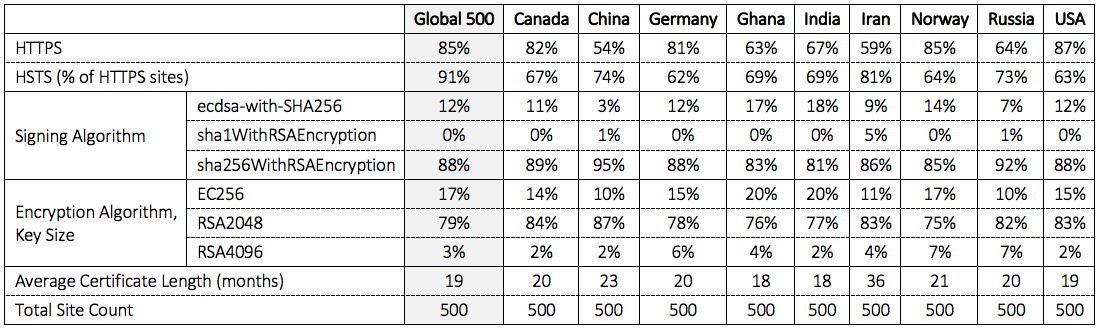
\includegraphics[width=\textwidth]{final_results.png}
	\caption{Results per country.}
	\label{fig:results}
	\end{centering}
\end{figure}

\begin{figure}[tb]
	\begin{centering}
	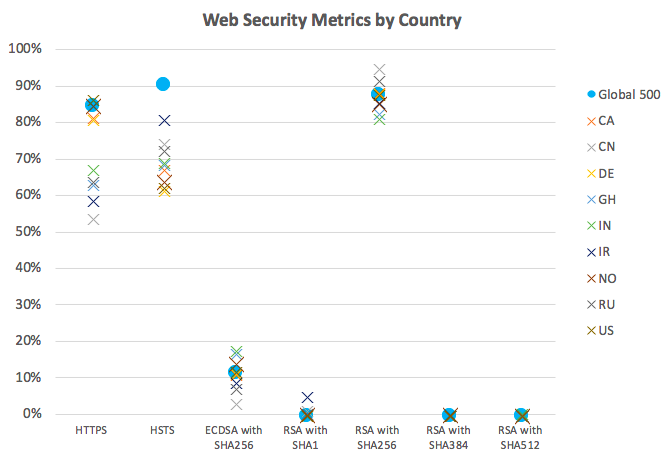
\includegraphics[width=11cm]{security.png}
	\caption{Security parameters.}
	\label{fig:security}
	\end{centering}
\end{figure}

\subsection{Certificate Issuance}

Here, we review the certificate data gathered from all of the unique 
sites scanned (3221 unique sites out of 4500 total scanned). We find 
that the certificates are typically issued for one, two, or 
three years, though we do see shorter periods of three or six months. 
Several certificates issued in China and Iran were valid for 30 to 100 
years, but these was marked as insecure in major browsers.

The graphs in Figure 3 visualize the number of certificates that have 
been issued, how many are expiring soon and how long they are valid 
after the issue date. We mark the dates when Google and Mozilla released
browser security announcements in the left-most figure. As Google and 
Mozilla begin rolling out strict warnings for insecure websites, we see 
that an increasing number of websites are issued new certificates.

The sharp increase in new certificates issued after the browser 
announcements suggests that many websites recently updated their 
certificates or were issued their first one. Future analysis will 
account for coinciding factors that may also have contributed to these 
trends, but our results thus far support the claim that Google and 
Mozilla's initiatives are successfully impacting the security culture 
among the top websites.

\begin{figure}[!htb]
    \begin{centering}
    \minipage{0.32\textwidth}
        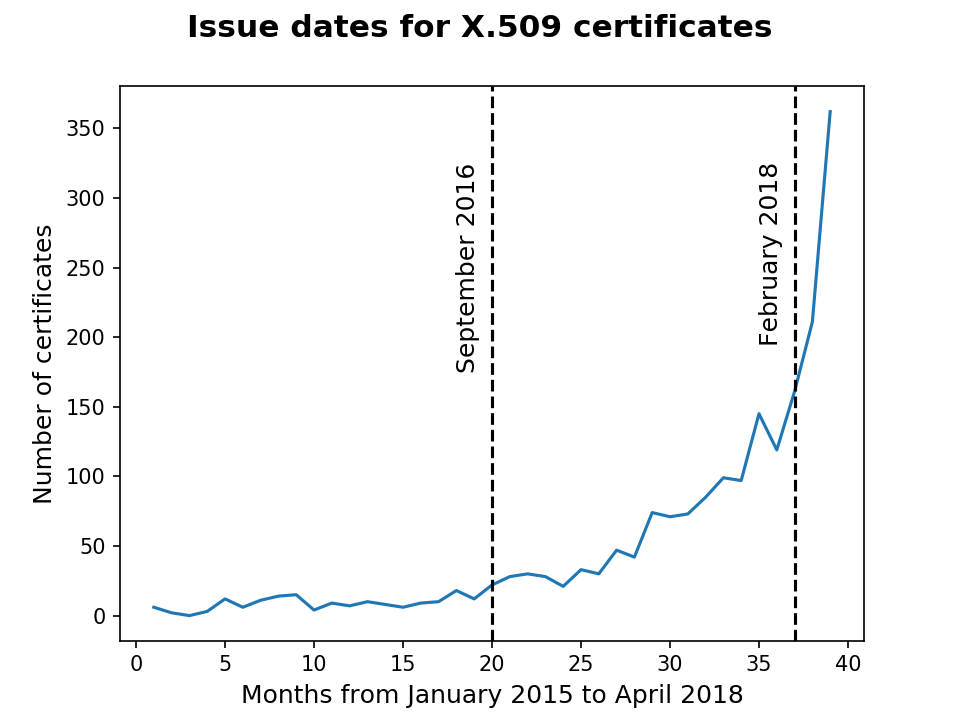
\includegraphics[width=\linewidth]{plot-issue.png}
    \endminipage\hfill
    \minipage{0.32\textwidth}
        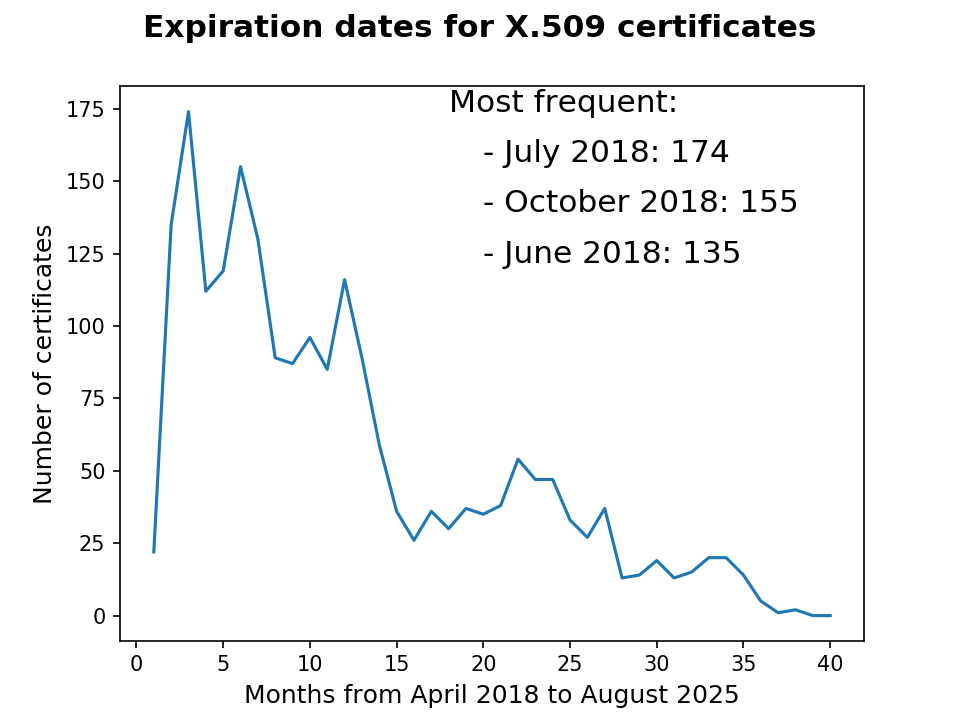
\includegraphics[width=\linewidth]{plot-expiration.png}
    \endminipage\hfill
    \minipage{0.32\textwidth}%
        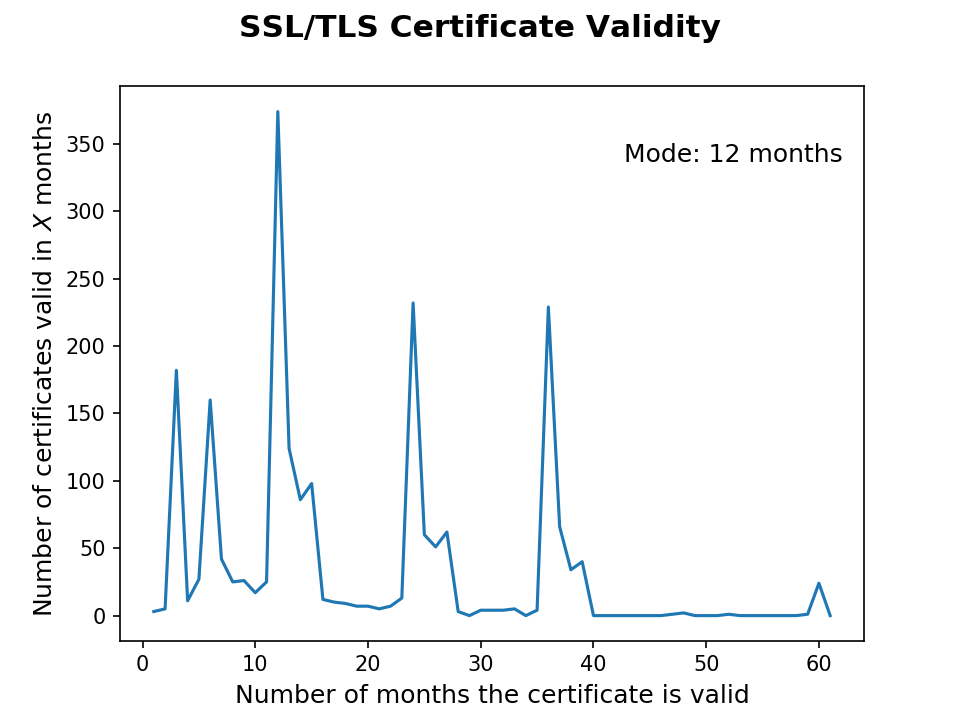
\includegraphics[width=\linewidth]{plot-certificate_lengths.png}
    \endminipage
    \caption{Certificate overview.}
	\label{fig:certificates}
    \end{centering}
\end{figure}

%----------------------------------------------------------------

\section{Limitations}

Our work is necessarily limited by the sample of sites we examine. As 
Scheitle et al. \cite{internettoplists} document, it is unclear how 
representative Alexa listings are of the entire web, as they are based 
on data collected from opt-in browser extensions. Though we considered 
alternate site listings provided by Quantcast and Majestic Million, we 
settled upon Alexa listings due to their stratification by country. 
Other listings typically require paid subscriptions. 

We manually verified a subset of websites with valid certificates and 
websites with errors, and found both false positive and false negative 
results compared with the Python script. We plan to test whether a 
purely OpenSSL solution would give different results on the same top 500
lists. It is also possible to use other programming languages such as 
JavaScript. We hope these next steps can give us both more accurate data
and also more insight into which algorithms are used for the symmetric 
key cryptography component of TLS, and the lengths of their security 
parameters.

Future work will attempt to distinguish between locally generated 
content and foreign content to better understand local capacity for 
implementing TLS, and assess the relationship between site popularity 
and security. We will also study HSTS more in detail to achieve more 
accurate result, in addition to check the availability of certificate 
revocation information and the certificate transparency for the 
different web pages of interest.

%----------------------------------------------------------------

\section{Conclusion}

We scanned the top five hundred websites accessed by internet users from
nine countries to paint a disaggregated portrait of web security. This 
contrasts with existing scans that evaluate the entire address space or 
specific sectors. Our results show significant regional variation and 
suggest that users from China, Ghana, Iran, and Russia are relatively 
more susceptible to eavesdropping or corrupted data when sending 
information over the internet. Future work will expand the sample of 
countries considered to assess broader regional patterns in security. 
These initial results suggest that while web security is improving, the 
benefits are not yet evenly distributed globally. Knowledge of where the
web is insecure, as experienced by a country's users, can help policy 
makers and other stakeholders place targeted pressure on the sites in 
question to implement HTTPS and HSTS, or recommend stronger encryption 
algorithms. 

Thus far, the majority of action incentivizing web security has come 
from private sector actors, as we've seen in the success of browser 
policies and cost-decreasing initiatives such as Let's Encrypt. As 
Google and Mozilla begin to mark websites without HTTPS as insecure, it 
will be interesting to see how these results evolve. We expect the 
percentage of websites using HTTPS to increase significantly in the 
coming months, given past responsiveness to browser policy. 

\bibliographystyle{plain}
\bibliography{easychair}

\end{document}